\section{Algorithm}


\begin{algorithm}
  \caption{\hskip0.5em Gilbert2D($p$, $\alpha$, $\beta$) }
  \label{alg:gilbert2d}
  \begin{algorithmic}
    \State \textbf{Input:} $p, \alpha, \beta \in \mathbb{Z}^3$
    %\State \textbf{Input:} $p \in \mathbb{N}^3$, \Comment{ start position}
    %\State \textbf{Input:} $\alpha \in \mathbb{N}^3$,  \Comment{"width" like axis}
    %\State \textbf{Input:} $\beta \in \mathbb{N}^3$,  \Comment{"height" like axis}

    \State $\alpha_2 = \alpha // 2$
    \State $\beta_2 = \beta // 2$

    \If{ $(|\beta| \equiv 1)$ }
      \ForAll{ $i \in |\alpha|$ }
        \State \textbf{yield} $p + i \cdot \delta(\alpha)$
      \EndFor
    \ElsIf{ $(|\alpha| \equiv 1)$ }
      \ForAll{ $i \in |\beta|$ }
        \State \textbf{yield} $p + i \cdot \delta(\alpha)$
      \EndFor
    \ElsIf{ $(2 |\alpha| > 3 |\beta|)$ }
      \If{ $(|\alpha_2| > 2)$ and $(|\alpha_2| \bmod{2} \equiv 1)$ }
        \State $\alpha_2 \leftarrow \alpha_2 + \delta(\alpha)$
      \EndIf
      \State \textbf{yield} Gilbert2D($p$, $\alpha_2$, $\beta$)
      \State \textbf{yield} Gilbert2D($p + \alpha_2$, $\alpha - \alpha_2$, $\beta$)
    \Else
      \If{ $(|\beta_2| > 2)$ and $(|\beta_2| \bmod{2} \equiv 1)$ }
        \State $\beta_2 \leftarrow \beta_2 + \delta(\beta)$
      \EndIf
      \State \textbf{yield} Gilbert2D($p$, $\beta_2$, $\alpha_2$)
      \State \textbf{yield} Gilbert2D($p + \beta_2$, $\alpha$, $\beta - \beta_2$)
      \State $p' \leftarrow p + \alpha - \delta(\alpha) + \beta_2 - \delta(\beta)$
      \State \textbf{yield} Gilbert2D($p'$, $\beta_2$, $-(\alpha - \alpha_2)$)
    \EndIf
  \end{algorithmic}
\end{algorithm}

\floatname{algorithm}{Procedures}

\begin{algorithm}
  \caption{ \hskip0.5em S-Split functions (eccentric splits) }
  \label{alg:eccentric3d}
  \begin{algorithmic}

    \State
    \State \textit{\# split halfway on $\alpha$ }
    \Function{$S_0$}{$p$, $\alpha$, $\beta$, $\gamma$}
      \State $\alpha_2 \leftarrow (\alpha // 2)$
      \If{ $(|\alpha| > 2)$ and $((|\alpha_2| \bmod{2}) \equiv 1)$ }
        \State $\alpha_2 \leftarrow \alpha_2 + \delta(\alpha)$
      \EndIf
      \State \textbf{yield} Gilbert3D($p$, \\ \hskip8.25em $\alpha_{2}$, $\beta$, $\gamma$ )
      \State \textbf{yield} Gilbert3D($p + \alpha_{2}$, \\ \hskip8.25em $(\alpha - \alpha_{2})$, $\beta$, $\gamma$ )
    \EndFunction

    \State
    \State \textit{\# split $\frac{1}{3}$ on $\gamma$ and halfway on $\alpha$ }
    \Function{$S_1$}{$p$, $\alpha$, $\beta$, $\gamma$}
      \State $\alpha_2, \gamma_3 \leftarrow (\alpha // 2), (\gamma // 3)$
      \If{ $(|\alpha| > 2)$ and $((|\alpha_2| \bmod{2}) \equiv 1)$ }
        \State $\alpha_2 \leftarrow \alpha_2 + \delta(\alpha)$
      \EndIf
      \If{ $(|\gamma| > 2)$ and $((|\gamma_3| \bmod{2}) \equiv 1)$ }
        \State $\gamma_3 \leftarrow \gamma_3 + \delta(\gamma)$
      \EndIf
      \State \textbf{yield} Gilbert3D($p$, \\ \hskip8.25em $\gamma_3$, $\alpha_2$, $\beta$)
      \State \textbf{yield} Gilbert3D($p + \gamma_3$, \\ \hskip8.25em $\alpha$, $\beta$, $(\gamma - \gamma_3)$)
      \State \textbf{yield} Gilbert3D($p + \alpha - \delta(\alpha) + \gamma_{3} - \delta(\gamma)$, \\ \hskip8.25em $\gamma_3$, $(\alpha - \alpha_2)$, $\beta$)
    \EndFunction

    \State
    \State \textit{\# split $\frac{1}{3}$ on $\beta$ and halfway on $\alpha$ }
    \Function{$S_2$}{$p$, $\alpha$, $\beta$, $\gamma$}
      \State $\alpha_2, \beta_3 \leftarrow (\alpha // 2), (\beta // 3)$
      \If{ $(|\alpha| > 2)$ and $((|\alpha_2| \bmod{2}) \equiv 1)$ }
        \State $\alpha_2 \leftarrow \alpha_2 + \delta(\alpha)$
      \EndIf
      \If{ $(|\beta| > 2)$ and $((|\beta_3| \bmod{2}) \equiv 1)$ }
        \State $\beta_3 \leftarrow \beta_3 + \delta(\beta)$
      \EndIf
      \State \textbf{yield} Gilbet3D($p$, \\ \hskip8.25em $\beta_{3}$, $\gamma$, $\alpha_2$ )
      \State \textbf{yield} Gilbet3D($p + \beta_{3}$, \\ \hskip8.25em $\alpha$, $(\beta - \beta_{3})$, $\gamma$ )
      \State \textbf{yield} Gilbet3D($p + \alpha - \delta(\alpha) + \beta_{3} - \delta(\beta)$, \\ \hskip8.25em $-\beta_{3}$, $\gamma$, $-\alpha$)
    \EndFunction

  \end{algorithmic}
\end{algorithm}

\begin{algorithm}
  \caption{ \hskip0.5em J-Split functions }
  \label{alg:eccentric3d}
  \begin{algorithmic}

    \State
    \State \textit{\# $|\gamma|$ even }
    \Function{$J_0$}{$p$, $\alpha$, $\beta$, $\gamma$}
      \State ok
    \EndFunction

    \State
    \State \textit{\# $|\gamma|$ odd, one of $|\alpha|$ or $|\beta|$ even }
    \Function{$J_1$}{$p$, $\alpha$, $\beta$, $\gamma$}
      \State ok
    \EndFunction

    \State
    \State \textit{\# $|\alpha|, |\beta|, |\gamma|$ odd }
    \Function{$J_2$}{$p$, $\alpha$, $\beta$, $\gamma$}
      \State ok
    \EndFunction

  \end{algorithmic}
\end{algorithm}

\floatname{algorithm}{Algorithm}

\begin{algorithm}
  %\caption{Gilbert3D($p \in \mathbb{Z}^3$, $\alpha \in \mathbb{Z}^3$, $\beta \in \mathbb{Z}^3$, $\gamma \in \mathbb{Z}^3$)}
  \caption{ \hskip0.5em Gilbert3D($p$, $\alpha$, $\beta$, $\gamma$) \\ \hskip3.0em $p, \alpha, \beta, \gamma \in \mathbb{Z}^3$ }
  \label{alg:gilbert3d}
  \begin{algorithmic}

%    \State
%    \State $\alpha_2, \beta_2, \gamma_2 \leftarrow (\alpha // 2), (\beta // 2), (\gamma // 2) $
%
%    \State
%    \State // \textit{ Prefer even, except special consideration for $\alpha$ }
%    \State \textbf{if} ($(|\alpha| > 2)$ and $((|\gamma| \bmod{2}) \cdot (|\alpha_2| \bmod{2}) \equiv 1)$)
%      \State \hskip1.5em $\alpha_2 \leftarrow \alpha_2 + \delta(\alpha_2)$
%    \State $\beta_2 + \delta(\beta)$ \textbf{if} $(|\beta_2| > 2)$ and $(|\beta_2| \bmod{2} \equiv 1)$
%    \State $\gamma_2 + \delta(\gamma)$ \textbf{if} $(|\gamma_2| > 2)$ and $(|\gamma_2| \bmod{2} \equiv 1)$
    \State
    \State\textit{\# Parity of dimensions}
    \State $\alpha_0,\beta_0,\gamma_0 \leftarrow (|\alpha|\bmod{2}),(|\beta|\bmod{2}),(|\gamma|\bmod{2})$

    \State
    \State\textit{\# Base cases }
    \State \textbf{if} ($(|\alpha|\equiv 2)$ and $(|\beta|\equiv 2)$ and $(|\gamma| \equiv 2)$)
    \State \hskip1.5em \Return Hilbert3D($p$,$\alpha$,$\beta$,$\gamma$) 
    \State \Return Gilbert2D($p$,$\beta$,$\gamma$) \textbf{if} $(|\alpha| \equiv 1)$
    \State \Return Gilbert2D($p$,$\alpha$,$\gamma$) \textbf{if} $(|\beta| \equiv 1)$
    \State \Return Gilbert2D($p$,$\alpha$,$\beta$) \textbf{if} $(|\gamma| \equiv 1)$

    \State
    \State\textit{\# Eccentric cases }
    \State \Return $S _ 0$($p$,$\alpha$,$\beta$,$\gamma$) \textbf{if}$(3 |\alpha|>5|\beta|)\text{and}(3|\alpha|>5|\gamma|))$
    \State \Return $S _ 2$($p$,$\alpha$,$\beta$,$\gamma$) \textbf{if}$(2 |\beta| > 3 |\gamma|)\text{or}(2 |\beta| > 3 |\alpha|))$
    \State \Return $S _ 1$($p$,$\alpha$,$\beta$,$\gamma$) \textbf{if}$(2 |\gamma| > 3 |\beta|)$

%    \If{ $((3 |\alpha| > 5 |\beta|) \text{ and } (3 |\alpha| > 5 |\gamma|))$ }
%      \State \Return $S _ 0$( $p$, $\alpha$, $\beta$, $\gamma$ )
%      %\State \textbf{yield} Gilbert3D( $p$, $\alpha_{2}$, $\beta$, $\gamma$ )
%      %\State \Return Gilbert3D( $(p + \alpha_{2})$, $(\alpha - \alpha_{2})$, $\beta$, $\gamma$ )
%    \ElsIf{ $((2 |\beta| > 3 |\gamma|) \text{ or } (2 |\beta| > 3 |\alpha|))$ }
%      \State \Return $S _ 2$( $p$, $\alpha$, $\beta$, $\gamma$ )
%      %\State \textbf{yield} Gilbet3D( $p$, $\beta_{3}$, $\gamma$, $\alpha_2$ )
%      %\State \textbf{yield} Gilbet3D( $p + \beta_{3}$, $\alpha$, $\beta - \beta_{3}$, $\gamma$ )
%      %\State $p' \leftarrow  p + \alpha - \delta(\alpha) + \beta_{3} - \delta(\beta)$
%      %\State \Return Gilbet3D( $p'$, $-\beta_{3}$, $\gamma$, $-\alpha$ )
%    \ElsIf{ $(2 |\gamma| > 3 |\beta|)$ }
%      \State \Return $S _ 1$( $p$, $\alpha$, $\beta$, $\gamma$ )
%      %\State \textbf{yield} Gilbert3D( $p$, $\gamma_3$, $\alpha_2$, $\beta$ )
%      %\State \textbf{yield} Gilbert3D( $p + \gamma_3$, $\alpha$, $\beta$, $\gamma - \gamma_3$ )
%      %\State $p' \leftarrow  p + \alpha - \delta(\alpha) + \gamma_{3} - \delta(\gamma)$
%      %\State \Return Gilbert3D( $p'$, $\gamma_3$, $\alpha - \alpha_2$, $\beta$ )
%    \EndIf

    \State
    \State \textit{\# Bulk recursion }
    \State \Return $J _ 0$($p$,$\alpha$,$\beta$,$\gamma$) \textbf{if} $(\gamma_0 \equiv 0)$
    \State \Return $J _ 1$($p$,$\alpha$,$\beta$,$\gamma$) \textbf{if} $(\alpha_0 \equiv 0)$or$(\beta_0\equiv 0)$
    \State \Return $J _ 2$($p$,$\alpha$,$\beta$,$\gamma$)

%    \If{ $((|\alpha| \bmod{2}) (|\beta| \bmod{2}) (|\gamma| \bmod{2}) \equiv 1)$ }
%
%      \State \Return $J _ 2$( $p$, $\alpha$, $\beta$, $\gamma$ )
%
%      %\State \textbf{yield} Gilbert3D( $p$, $\beta_2$, $\gamma$, $\alpha_2$ )
%      %\State \textbf{yield} Gilbert3D( $p+\beta_2$, $\gamma_2$, $\alpha$, $\beta - \beta_2$ )
%      %\State \textbf{yield} Gilbert3D( $p+\beta_2 + \gamma_2$, $\alpha$, $\beta - \beta_2$, $\gamma - \gamma_2$ )
%      %\State $p' \leftarrow p + \alpha - \delta(\alpha) + \beta_2 - \delta(\beta) + \gamma_2$
%      %\State \textbf{yield} Gilbert3D($p'$, $-\beta_2$, $\gamma- \gamma_2$, $-(\alpha - \delta(\alpha))$ )
%      %\State $p' \leftarrow p + \alpha - \delta(\alpha) + \gamma_2 - \delta(\gamma)$
%      %\State \Return Gilbert3D( $p'$, $-\gamma_2$, $-(\alpha - \alpha_2)$, $\beta_2$ )
%
%    \ElsIf{ $((|\gamma| \bmod 2) \equiv 1)$  }
%
%      \State \Return $J _ 1$( $p$, $\alpha$, $\beta$, $\gamma$ )
%
%      %\State \textbf{yield} Gilbert3D( $p$, $\gamma2$, $\alpha_2$, $\beta_2$ )
%      %\State \textbf{yield} Gilbert3D( $p+\gamma_2$, $\beta$, $\gamma - \gamma_2$, $\alpha_2$ )
%      %\State $p' \leftarrow p + \gamma_2 - \delta(\gamma) + \beta - \delta(\beta)$
%      %\State \textbf{yield} Gilbert3D( $p'$, $\alpha$, $-(\beta - \beta_2)$, $-\gamma_2$ )
%      %\State $p' \leftarrow p + \alpha - \delta(\alpha) + \beta - \delta(\beta) + \gamma_2 - \delta(\gamma)$
%      %\State \textbf{yield} Gilbert3D( $p'$, $\beta$, $\gamma - \gamma_2$, $-(\alpha - \alpha_2)$ )
%      %\State $p' \leftarrow p + \alpha - \delta(\alpha) + \gamma_2 - \delta(\gamma)$
%      %\State \Return Gilbert3D( $p'$, $-\gamma_2$, $-(\alpha - \alpha_2)$, $\beta_2$ )
%    \EndIf
%
%    \State \Return $J _ 0$( $p$, $\alpha$, $\beta$, $\gamma$ )
%
%    %\State
%    %\State \textbf{yield} Gilbert3D( $p$, $\beta_2$, $\gamma_2$, $\alpha_2$ )
%    %\State \textbf{yield} Gilbert3D( $p+\beta_2$, $\gamma$, $\alpha_2$, $\beta - \beta_2$ )
%    %\State $p' \leftarrow p + \beta_2 - \delta(\beta_2) + \gamma - \delta(\gamma)$
%    %\State \textbf{yield} Gilbert3D( $p'$, $\alpha$, $-\beta_2$, $-(\gamma - \gamma_2)$ )
%    %\State $p' \leftarrow p + \alpha - \delta(\alpha) + \beta_2 + \gamma - \delta(\gamma)$
%    %\State \textbf{yield} Gilbert3D( $p'$, $-\gamma$, $-(\alpha - \alpha_2)$, $\beta - \beta_2$ )
%    %\State $p' \leftarrow p + \alpha - \delta(\alpha) + \beta_2 - \delta(\beta)$
%    %\State \Return Gilbert3D( $p'$, $-\beta_2$, $\gamma_2$, $-(\alpha - \alpha_2)$ )

  \end{algorithmic}
\end{algorithm}

\begin{figure}[h]
  \centering
  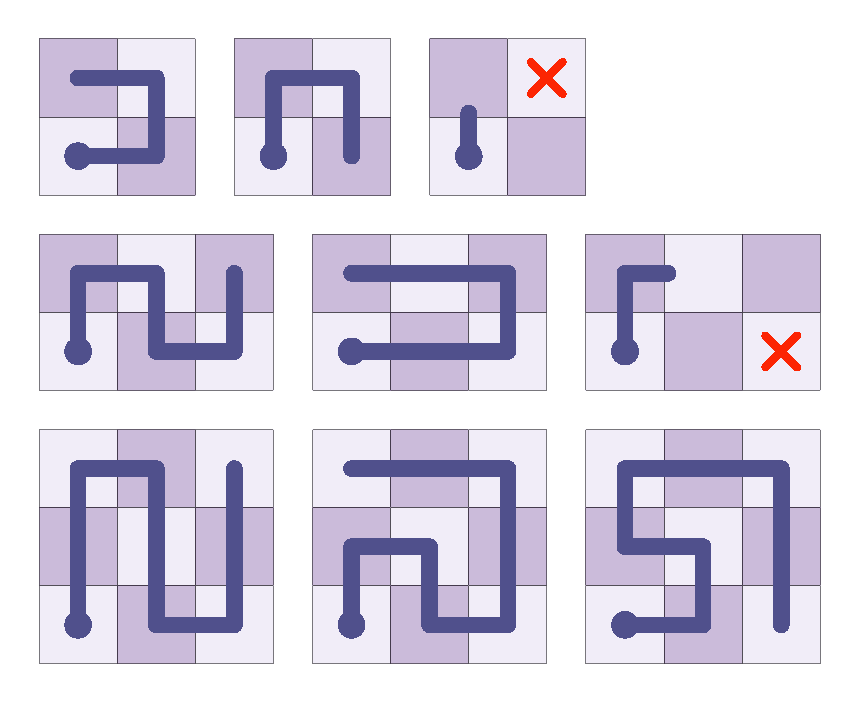
\includegraphics[width=\linewidth]{simple_hampath.pdf}
  \caption{ Illustrative examples of Hamiltonian paths height/width that are even/even, even/odd and odd/odd, respectively,
            when starting from the lower left hand corner }
  \label{fig:exampleHampath}
\end{figure}


\begin{figure}[h]
  \centering
  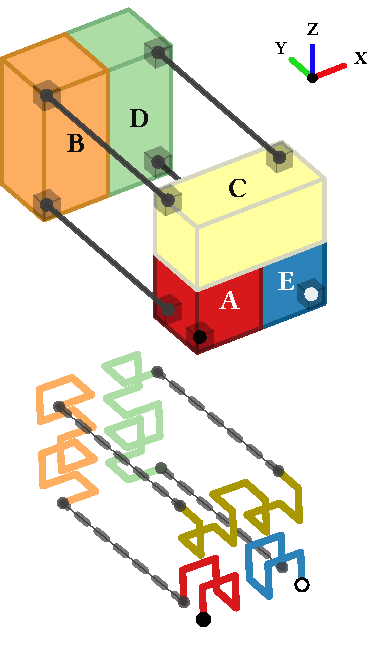
\includegraphics[width=\linewidth]{gilbert3d_explode.pdf}
  \caption{ The J-split subdivision, representing the main subdivision of the build recursion for the 3D Gilbert curve case }
  \label{fig:gilbert3DJSplit}
\end{figure}


\begin{figure*}[ht]
  \centering
  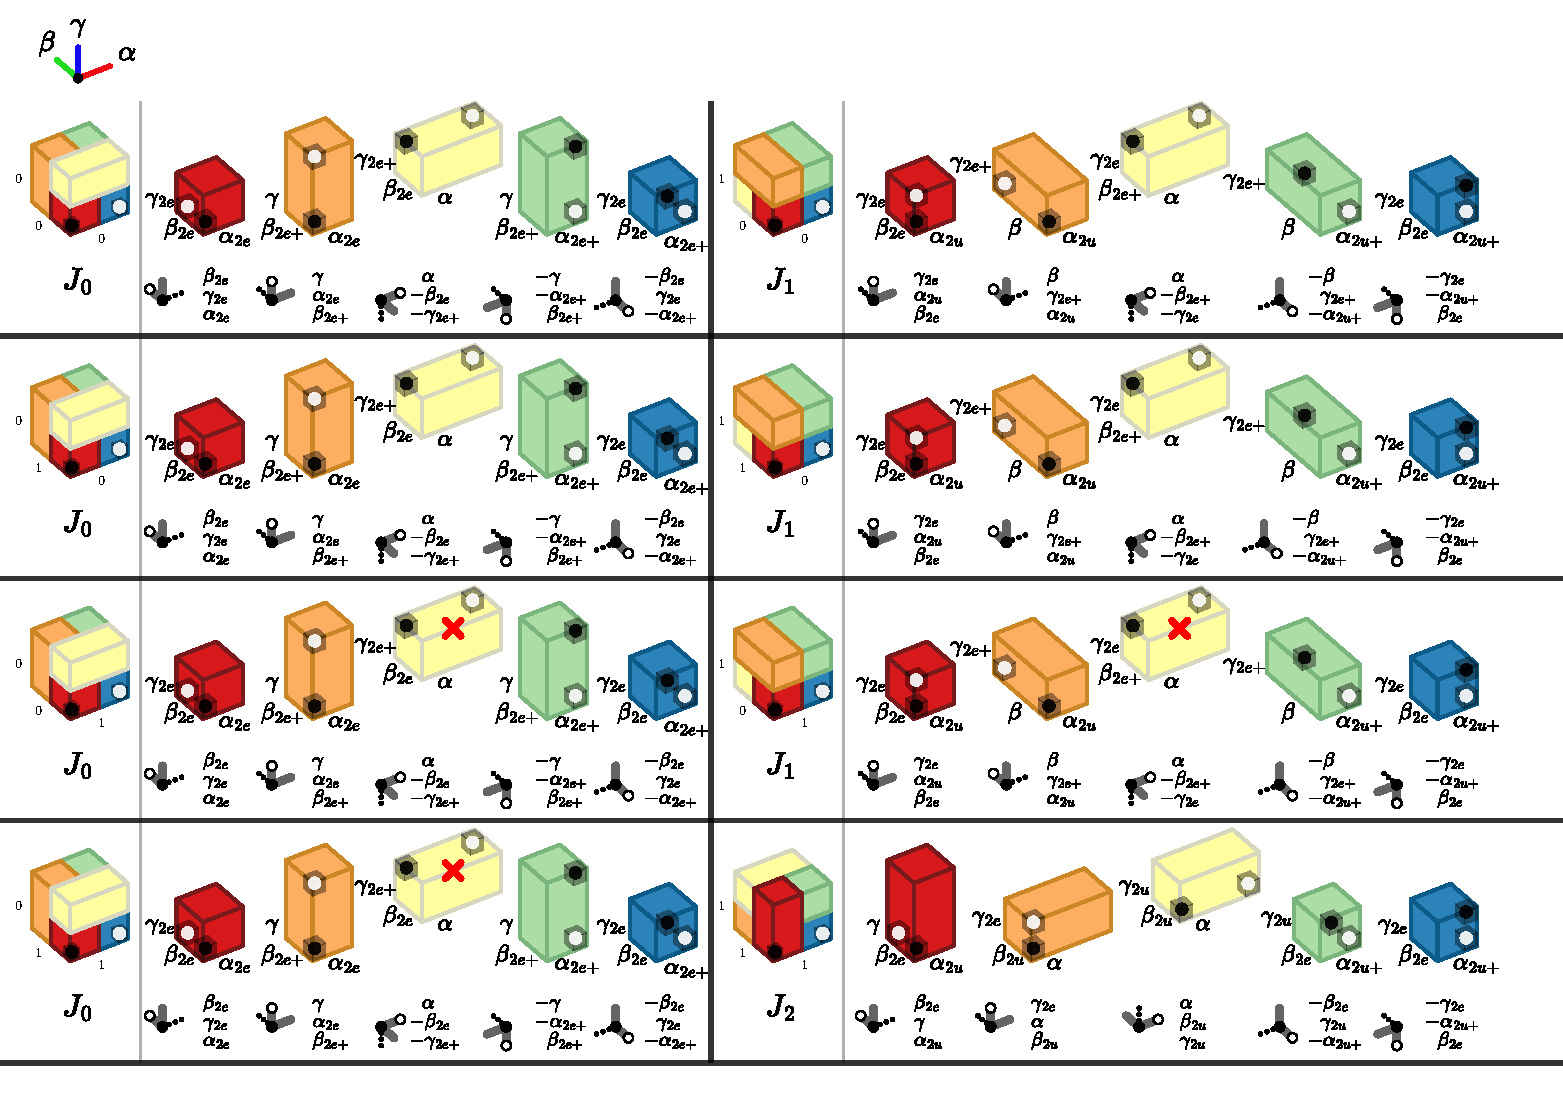
\includegraphics[width=\textwidth]{gilbert3d_case.pdf}
  \caption{ Bulk recursion J-split atlas for the 3D Gilbert algorithm }
  \label{fig:gilbert3DCase}
\end{figure*}



